% File name: report/technicalabstract.tex

\documentclass[a4paper,11pt]{article}  % Standard document class
\usepackage[english]{babel}            % Set document language
\usepackage{fullpage}                  % Set up page for small margins etc
\usepackage{listings}
\usepackage{graphicx}                  % For including images in document

\usepackage{tikz}
\usetikzlibrary{shapes,arrows}

\usepackage{appendix}
\usepackage{color}
\usepackage{hyperref}

\usepackage{caption}
\usepackage{subcaption}

%\usepackage{placeins}                  % Allows use of \FloatBarrier
% to avoid images or tables
% moving into next section
%\usepackage{subfig}                    % For subfigures...

\usepackage{amsmath}                   % For improving maths/formula typesetting
%\usepackage{tabular}                  % Table changing package

%\usepackage{algpseudocode}             % For producing algorithms/flowcharts

\usepackage{listings}                  % For including source code in document
\lstset{
  basicstyle = \small
}

% Provide command for scientific notation
\providecommand{\e}[1]{\ensuremath{\times10^{#1}}}
\providecommand{\degrees}{\ensuremath{^{\circ}}}

\setlength{\parindent}{0in}
\setlength{\parskip}{\baselineskip}%


% Define title here:
\title{4th Year Project: Automated soldering/solder paste machine (C-PJGL2-7) \\ Technical Abstract} %C-PJGL2-7
%\title{4th Year Project: Automated soldering/solder paste machine (C-PJGL2-7) \\ \vspace{2 mm} {\large Technical Abstract}}
\author{James Glanville (EM)}
\date{11th June 2013}

\hypersetup{
    colorlinks,
    allcolors=blue,
    linktoc=all,
}

\begin{document}

% generate title
\maketitle

%\begin{figure}[ht!]
%\centering
%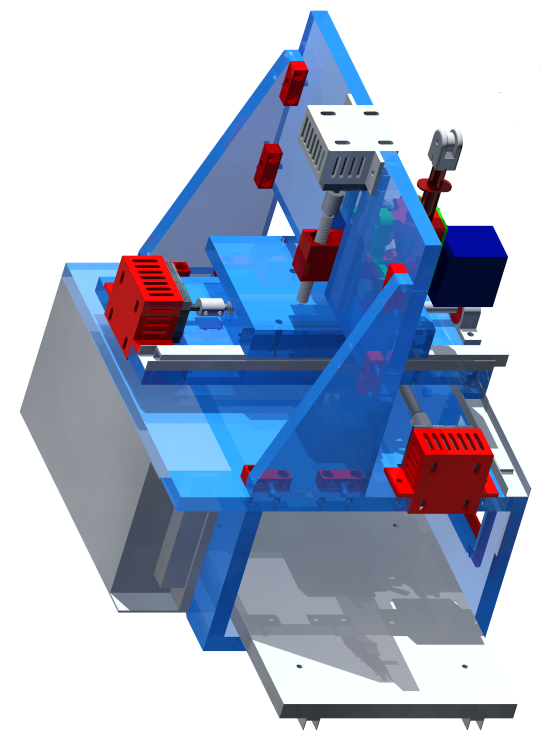
\includegraphics[width=100mm]{resources/render.png}
%\label{render}
%\end{figure}


\section*{Project Summary}
The aim of the project was to develop a tool to assist the process of 
producing boards with surface mount components. The main problems that
were the focus of the project brief were:

\begin{itemize}\itemsep0em
\item
How to place components accurately on to the board.
\item
How to solder them in place.
\end{itemize}

Two further goals were added during the course of the project:

\begin{itemize}\itemsep0em
\item
The ability to produce the PCB itself.
\item
The ability to drill any holes for through-hole components and vias, as
well as routing out the board outline.
\end{itemize}

\section*{Project Approach}
It was decided to build a three-axis CNC machine with a number of interchangeable
tools which collectively could support all the required functions.

The three-axis system uses commonly-available drawer slides as a novel
and inexpensive slide mechanism. Small stepper motors coupled to threaded
rod are used for actuation. An attempt was made during the design phase
to have the three axis as similar as possible, a "generic unit", that would
simplify design and ensure all errors and calculations were the same.

A number of tools were constructed to perform the various actions:

\begin{itemize}\itemsep0em
\item
A spindle that would accept both milling and drilling bits. A novel design
was used that surrounded the bit with small ball bearings. The bit was loosely
coupled to a brushless motor, so that only rotational motion was transferred.
In this way both run-out and cost were both reduced compared to a more
traditional spindle.
\item
A solder paste extruder was designed to accurately dispense small volumes
of solder paste from the syringes in which it is commonly supplied.
\item
A vacuum needle tool was designed to pick and place the surface mount
components. This has an integral pressure sensor to detect the presence of
a component.
\item
A hot air tool was designed to heat and reflow the solder paste when the board
was populated.
\end{itemize}

\section*{Report Structure}
The structure of the report is as follows:

\begin{itemize}\itemsep0em
\item
Detailed description of project goals. This section explains the project
brief along with suggested enhancements.
\item
Project approach. The methodology used in the project is discussed and 
chosen.
\item
Design possibilities. Various designs for the machine are considered.
\item
Chosen design. The design is chosen from those considered.
\item
Manufacture and testing. The machine as designed is evaluated.
\item
Improved designs. The machine is improved with the feedback from the initial testing stage.
\item
Results and Conclusions. The machine in its final form is evaluated.
\end{itemize}

\section*{Results and Conclusions}
The machine that was designed during the course of the project has proven
to be capable of PCB manufacture and population. Some problems with
reliability are apparent, however the design shows promise and could be
improved with further work.

During testing it has been the author's conclusion that while the original
project goals have been proven to work, the pcb manufacturing aspect of the
project has not proved to be practical for the smallest of traces. This
does not present as much of a problem as it may appear, as boards with particularly fine
traces are likely to need several layers and therefore be impractical for
hobbyist manufacture.



\end{document}
